\section{Dataset generation}
\subsection{Tested approaches}
The deep learning approaches explained in this document are \textit{supervised learning} techniques that require a labeled dataset. Several paths were tested in order to generate this kind of dataset:
\begin{itemize}
    \item \emph{IMU sensors}: usage of gyroscope and accelerometer sensors of a smartphone to estimate the position of the camera during a video given a fixed origin point. 
    \item \emph{digital video}: usage of free online 3 dimensional datasets in which video can be recorder in a digital way.
    \item \emph{motion capture system}: usage of a motion capture system that estimates the camera position following some tracking objects attached to the subject.
    \item \emph{structure from motion techniques}: techniques that compute a sparse and dense reconstruction from a sequence of images.
\end{itemize}

The main problem encountered with IMU sensors was the high noise presents during acquisitions, the final signal was very dirty, and the resolution was not acceptable for the dataset generation. A possible solution could have been the usage of a well calibrated hardware used in other kind of contexts.

Most of the 3 dimensional acquisitions available online for free are acquired with \emph{depth sensors} or \emph{LIDAR sensors}, for this reason although the camera pose estimation would not have presented any errors the images would have been at low quality.

The motion capture system is able to follows the position of the tracked objects with extremely precision, the main problematic remains the associated of poses to video captured from the camera held by the tracked subject. Other difficulties involved the calibration of the tool.

The techniques of structure from motion were invented with the goal of generate structures for which a huge amount of photos is available. The overall idea is to feed the algorithm with data in order to extract feature and build a recomposition of the environment. A step required in order to obtain a result is the estimation of the pose of images. These intermediate requirement have been exploited by us to generate a labeled dataset.

\subsection{Pipeline}
The implemented pipeline require a video captured by any camera, it is not required any calibration of the sensor. It is composed by several steps:
\begin{enumerate}
    \item video split: the captured video is split into many frames; 
    \item structure from motion: images obtained from the previous step are fed into a structure motion tool called \emph{COLMAP};
    \item cross validation dataset: positions obtained during the camera estimation of the reconstruction process are split into three batches: train, validation, test.
\end{enumerate}

\begin{figure}[h]
    \begin{center}
        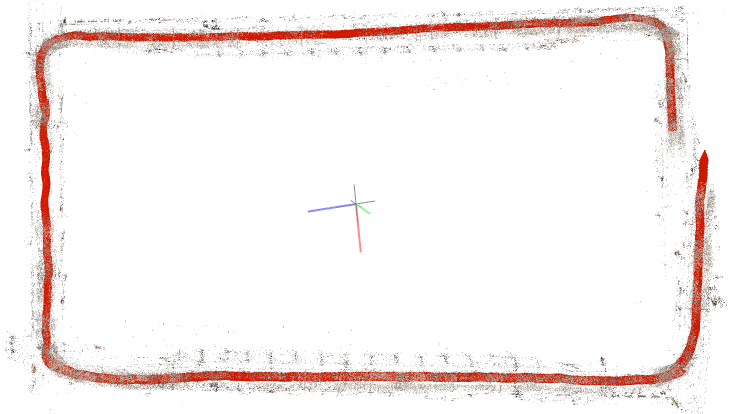
\includegraphics[width=0.45\textwidth]{./imgs/trajectory_colmap.png}
    \end{center}
    \caption{Trajectory computed by COLMAP}
    \label{fig:trajectory-colmap}
\end{figure}

In \cref{fig:trajectory-colmap} is presented the trajectory obtained with the structure from motion techinque through COLMAP. The process involes a feature extraction phase, elements obtained are shown in \cref{fig:features-colmap}.

\begin{figure}[h]
    \begin{center}
        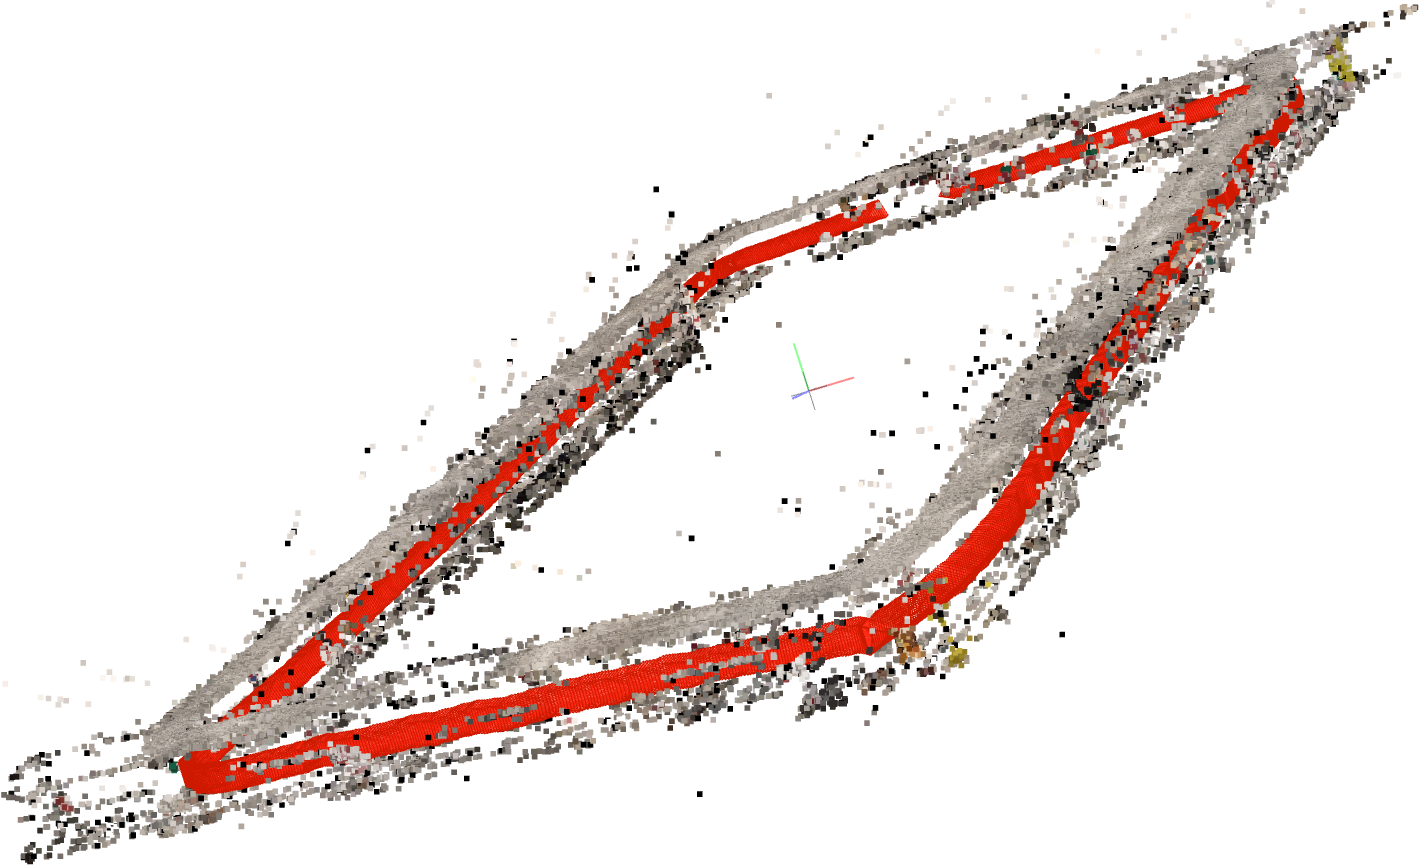
\includegraphics[width=0.45\textwidth]{./imgs/extracted_features_colmap.png}
    \end{center}
    \caption{Features extracted by COLMAP}
    \label{fig:features-colmap}
\end{figure}
